\documentclass[a4paper, 14pt]{extarticle}
\usepackage[settings]{markdown}
\usepackage{minted}

\usepackage{caption}
\usepackage{float}   


% Поля
%--------------------------------------
\usepackage{geometry}
\geometry{a4paper,tmargin=2cm,bmargin=2cm,lmargin=3cm,rmargin=1cm}
%--------------------------------------


%Russian-specific packages
%--------------------------------------
\usepackage[T2A]{fontenc}
\usepackage[utf8]{inputenc} 
\usepackage[english, main=russian]{babel}
%--------------------------------------

\usepackage{textcomp}

% Красная строка
%--------------------------------------
\usepackage{indentfirst}               
%--------------------------------------             


%Graphics
%--------------------------------------
\usepackage{graphicx}
\graphicspath{ {./images/} }
\usepackage{wrapfig}
%--------------------------------------

% Полуторный интервал
%--------------------------------------
\linespread{1.3}                    
%--------------------------------------

%Выравнивание и переносы
%--------------------------------------
% Избавляемся от переполнений
\sloppy
% Запрещаем разрыв страницы после первой строки абзаца
\clubpenalty=10000
% Запрещаем разрыв страницы после последней строки абзаца
\widowpenalty=10000
%--------------------------------------

%Списки
\usepackage{enumitem}

%Подписи
\usepackage{caption} 

%Гиперссылки
\usepackage{hyperref}

\hypersetup {
	unicode=true
}

%Рисунки
%--------------------------------------
\DeclareCaptionLabelSeparator*{emdash}{~--- }
\captionsetup[figure]{labelsep=emdash,font=onehalfspacing,position=bottom}
%--------------------------------------

\usepackage{tempora}
\usepackage{amsmath}
\usepackage{color}
\usepackage{listings}
\lstset{
  belowcaptionskip=1\baselineskip,
  breaklines=true,
  frame=L,
  xleftmargin=\parindent,
  language=Python,
  showstringspaces=false,
  basicstyle=\footnotesize\ttfamily,
  keywordstyle=\bfseries\color{blue},
  commentstyle=\itshape\color{purple},
  identifierstyle=\color{black},
  stringstyle=\color{red},
}

%--------------------------------------
%			НАЧАЛО ДОКУМЕНТА
%--------------------------------------

\begin{document}

%--------------------------------------
%			ТИТУЛЬНЫЙ ЛИСТ
%--------------------------------------
\begin{titlepage}
\thispagestyle{empty}
\newpage


%Шапка титульного листа
%--------------------------------------
\vspace*{-60pt}
\hspace{-65pt}
\begin{minipage}{0.3\textwidth}
\hspace*{-20pt}\centering

\includegraphics[width=\textwidth]{emblem}
\end{minipage}
\begin{minipage}{0.67\textwidth}\small \textbf{
\vspace*{-0.7ex}
\hspace*{-6pt}\centerline{Министерство науки и высшего образования Российской Федерации}
\vspace*{-0.7ex}
\centerline{Федеральное государственное бюджетное образовательное учреждение }
\vspace*{-0.7ex}
\centerline{высшего образования}
\vspace*{-0.7ex}
\centerline{<<Московский государственный технический университет}
\vspace*{-0.7ex}
\centerline{имени Н.Э. Баумана}
\vspace*{-0.7ex}
\centerline{(национальный исследовательский университет)>>}
\vspace*{-0.7ex}
\centerline{(МГТУ им. Н.Э. Баумана)}}
\end{minipage}
%--------------------------------------

%Полосы
%--------------------------------------
\vspace{-25pt}
\hspace{-35pt}\rule{\textwidth}{2.3pt}

\vspace*{-20.3pt}
\hspace{-35pt}\rule{\textwidth}{0.4pt}
%--------------------------------------

\vspace{1.5ex}
\hspace{-35pt} \noindent \small ФАКУЛЬТЕТ\hspace{50pt} <<Информатика и системы управления>>

\vspace*{-16pt}
\hspace{47pt}\rule{0.83\textwidth}{0.4pt}

\vspace{0.5ex}
\hspace{-35pt} \noindent \small КАФЕДРА\hspace{50pt} <<Теоретическая информатика и компьютерные технологии>>

\vspace*{-16pt}
\hspace{30pt}\rule{0.866\textwidth}{0.4pt}
  
\vspace{11em}

\begin{center}
\Large {\bf Лабораторная работа № 3} \\ 
\large {\bf по курсу <<Базы данных>>}\\
\end{center}\normalsize

\vspace{8em}


\begin{flushright}
  {Студент группы ИУ9-51Б Горбунов А. Д.\hspace*{15pt} \\
  \vspace{2ex}
  Преподаватель Вишняков И. Э.\hspace*{15pt}}
\end{flushright}

\bigskip

\vfill
 

\begin{center}
\textsl{Москва 2024}
\end{center}
\end{titlepage}
%--------------------------------------
%		КОНЕЦ ТИТУЛЬНОГО ЛИСТА
%--------------------------------------

\renewcommand{\ttdefault}{pcr}

\setlength{\tabcolsep}{3pt}
\newpage
\setcounter{page}{2}

\section{Задача}\label{Sect::task}
\par

\begin{enumerate}
    \item Преобразовать модель «сущность-связь», созданную в лабораторной работе №1, в реляционную модель согласно процедуре преобразования.
    \item Обосновать выбор типов данных, ключей, правил обеспечения ограничений минимальной кардинальности.
\end{enumerate}

\par

\section{Практическая реализация}\label{Sect::task}

Модель полученная в 1-й лабораторной работе:

\begin{figure}[H]
	\centering
	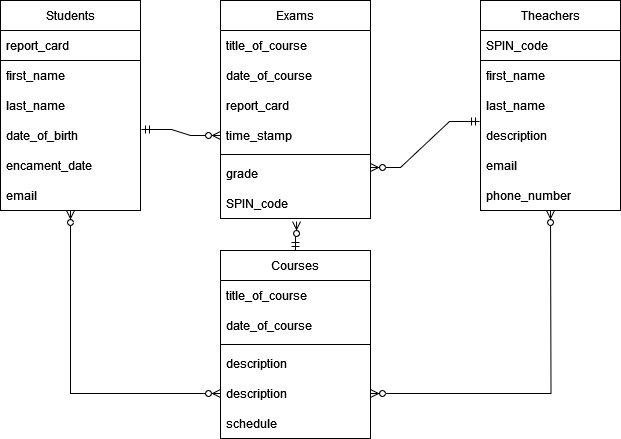
\includegraphics[width=0.8\textwidth]{scheme_lab1.png}
\caption{модель «сущность-связь»}
\label{fig:scheme}
\end{figure}

Результат 3-й лабораторной работы полученный в результате преобразований модели "сущность-связь" в реляционную:

\begin{figure}[H]
	\centering
	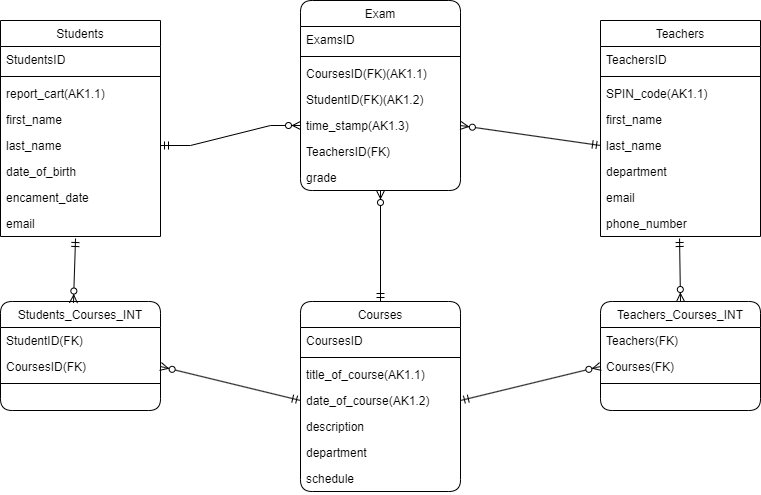
\includegraphics[width=0.8\textwidth]{scheme.png}
\caption{реляционная модель}
\label{fig:scheme}
\end{figure}
 
В таблицах 1-6 рассмотрены типы данных, на таблицах 7-13 рассмотрены ограничения для связи:

\begin{table}[H]
\centering
\captionsetup{singlelinecheck=false, justification=raggedright}
\caption{Students}
    \begin{tabular}
        {|c|c|c|c|c|}
        \hline
        Column Name & Type & Key & NULL Status  & Remarks \\
        \hline
        StudentsID & int & Primary Key & NOT NULL & Surrogate Key \\
        \hline
        report\_card & Char(10) & Alternate Key & NOT NULL & Unique (AK 1.1) \\
        \hline
        first\_name & Char(25) & No & NOT NULL &  \\
        \hline
        last\_name & Char(25) & No & NOT NULL &  \\
        \hline
        date\_of\_birth & DateTime & No & NOT NULL &  \\
        \hline
        encament\_date & DateTime & No & NULL &  \\
        \hline
        email & Char(25) & No & NOT NULL &  \\
    \hline
    \end{tabular}
\end{table}

\begin{table}[H]
\centering
\captionsetup{singlelinecheck=false, justification=raggedright}
\caption{Teachers}
    \begin{tabular}
        {|c|c|c|c|c|}
        \hline
        Column Name & Type & Key & NULL Status  & Remarks \\
        \hline
        TeachersID & int & Primary Key & NOT NULL & Surrogate Key \\
        \hline
        SPIN\_code & int & Alternate Key & NOT NULL & Unique (AK 1.1) \\
        \hline
        first\_name & Char(25) & No & NOT NULL &  \\
        \hline
        last\_name & Char(25) & No & NOT NULL &  \\
        \hline
        department & char(5) & No & NOT NULL &  \\
        \hline
        phone\_number & int & No & NOT NULL &  \\
        \hline
        email & Char(25) & No & NOT NULL &  \\
    \hline
    \end{tabular}
\end{table}

\begin{table}[H]
\centering
\captionsetup{singlelinecheck=false, justification=raggedright}
\caption{Courses}
    \begin{tabular}
        {|c|c|c|c|c|}
        \hline
        Column Name & Type & Key & NULL Status  & Remarks \\
        \hline
        CoursesID & int & Primary Key & NOT NULL & Surrogate Key \\
        \hline
        title\_of\_course & Char(25) & Alternate Key & NOT NULL & Unique (AK 1.1) \\
        \hline
        deta\_of\_course & DateTime & Alternate Key & NOT NULL & Unique (AK 1.2) \\
        \hline
        discription & varchar & No & NULL &  \\
        \hline
        department & char(5) & No & NOT NULL &  \\
        \hline
        schedule & varchar & No & NOT NULL &  \\
    \hline
    \end{tabular}
\end{table}

\begin{table}[H]
\centering
\captionsetup{singlelinecheck=false, justification=raggedright}
\caption{Students\_Courses\_INT}
    \begin{tabular}
        {|c|c|p{3cm}|c|p{3cm}|}
        \hline
        Column Name & Type & Key & NULL Status  & Remarks \\
        \hline
        StudentsID & int & Primary Key, Foreign Key & NOT NULL & Ссылается на "Students" \\
        \hline
        CoursesID & int & Primary Key, Foreign Key & NOT NULL & Ссылается на "Courses" \\
    \hline
    \end{tabular}
\end{table}

\begin{table}[H]
\centering
\captionsetup{singlelinecheck=false, justification=raggedright}
\caption{Teachers\_Courses\_INT}
    \begin{tabular}
        {|c|c|p{3cm}|c|p{3cm}|}
        \hline
        Column Name & Type & Key & NULL Status  & Remarks \\
        \hline
        TeacherID & int & Primary Key, Foreign Key & NOT NULL & Ссылается на "Teachers" \\
        \hline
        CoursesID & int & Primary Key, Foreign Key & NOT NULL & Ссылается на "Courses" \\
    \hline
    \end{tabular}
\end{table}

\begin{table}[H]
\centering
\captionsetup{singlelinecheck=false, justification=raggedright}
\caption{Exam}
    \begin{tabular}
        {|c|c|p{3cm}|c|p{4cm}|}
        \hline
        Column Name & Type & Key & NULL Status  & Remarks \\
        \hline
        ExamsID & int & Primary Key & NOT NULL & Surrogate Key \\
        \hline
        CoursesID & int & Alternate Key, Foreign Key & NOT NULL & Unique (AK 1.1),  Ссылается на "Courses" \\
        \hline
        StudentsID & int & Alternate Key, Foreign Key & NOT NULL & Unique (AK 1.2),  Ссылается на "Students" \\
        \hline
        time\_stamp & DateTime & Alternate Key & NOT NULL & Unique (AK 1.3) \\
        \hline
        TeachersID & int & Foreign Key & NOT NULL &  Ссылается на "Teachers" \\
        \hline
        grade & int & No & NOT NULL &  \\
    \hline
    \end{tabular}
\end{table}

\begin{table}[H]
\centering
\captionsetup{singlelinecheck=false, justification=raggedright}
\caption{Ограничение связи "Students - Students\_Courses\_INT"}
    \begin{tabular}
        {|p{4cm}|p{5cm}|p{5cm}|}
        \hline
        Действие & Ограничение на Students & Ограничение на Students\_Courses\_INT \\
        \hline
        Вставка & Без ограничений &  подбор родителя \\
        \hline
        Изменение первичного или внешнего ключа & запрещено & запрещено \\
        \hline
        Удаление & запрещено & запрещено \\
    \hline
    \end{tabular}
\end{table}

\begin{table}[H]
\centering
\captionsetup{singlelinecheck=false, justification=raggedright}
\caption{Ограничение связи "Courses - Students\_Courses\_INT"}
    \begin{tabular}
        {|p{4cm}|p{5cm}|p{5cm}|}
        \hline
        Действие & Ограничение на Courses & Ограничение на Students\_Courses\_INT \\
        \hline
        Вставка &  Без ограничений & подбор родителя \\
        \hline
        Изменение первичного или внешнего ключа & запрещено & запрещено \\
        \hline
        Удаление & запрещено & запрещено \\
    \hline
    \end{tabular}
\end{table}

\begin{table}[H]
\centering
\captionsetup{singlelinecheck=false, justification=raggedright}
\caption{Ограничение связи "Students - Exam"}
    \begin{tabular}
        {|p{4cm}|p{5cm}|p{5cm}|}
        \hline
        Действие & Ограничение на Students & Ограничение на Exam \\
        \hline
        Вставка &  Без ограничений & подбор родителя \\
        \hline
        Изменение первичного или внешнего ключа & запрещено & запрещено \\
        \hline
        Удаление & запрещено & запрещено \\
    \hline
    \end{tabular}
\end{table}

\begin{table}[H]
\centering
\captionsetup{singlelinecheck=false, justification=raggedright}
\caption{Ограничение связи "Courses - Exam"}
    \begin{tabular}
        {|p{4cm}|p{5cm}|p{5cm}|}
        \hline
        Действие & Ограничение на Courses & Ограничение на Exam \\
        \hline
        Вставка & Без ограничений & подбор родителя \\
        \hline
        Изменение первичного или внешнего ключа & запрещено & запрещено \\
        \hline
        Удаление & запрещено & запрещено \\
    \hline
    \end{tabular}
\end{table}

\begin{table}[H]
\centering
\captionsetup{singlelinecheck=false, justification=raggedright}
\caption{Ограничение связи "Courses - Teachers\_Courses\_INT"}
    \begin{tabular}
        {|p{4cm}|p{5cm}|p{5cm}|}
        \hline
        Действие & Ограничение на Courses & Ограничение на Teachers\_Courses\_INT \\
        \hline
        Вставка & Без ограничений & подбор родителя \\
        \hline
        Изменение первичного или внешнего ключа & запрещено & запрещено \\
        \hline
        Удаление & запрещено & запрещено \\
    \hline
    \end{tabular}
\end{table}

\begin{table}[H]
\centering
\captionsetup{singlelinecheck=false, justification=raggedright}
\caption{Ограничение связи "Teachers - Teachers\_Courses\_INT"}
    \begin{tabular}
        {|p{4cm}|p{5cm}|p{5cm}|}
        \hline
        Действие & Ограничение на Teachers & Ограничение на Teachers\_Courses\_INT \\
        \hline
        Вставка & Без ограничений & подбор родителя \\
        \hline
        Изменение первичного или внешнего ключа & запрещено & запрещено \\
        \hline
        Удаление & запрещено & запрещено \\
    \hline
    \end{tabular}
\end{table}

\begin{table}[H]
\centering
\captionsetup{singlelinecheck=false, justification=raggedright}
\caption{Ограничение связи "Teachers - Exam"}
    \begin{tabular}
        {|p{4cm}|p{5cm}|p{5cm}|}
        \hline
        Действие & Ограничение на Teachers & Ограничение на Exam \\
        \hline
        Вставка &  Без ограничений & подбор родителя \\
        \hline
        Изменение первичного или внешнего ключа & запрещено & запрещено \\
        \hline
        Удаление & запрещено & запрещено \\
    \hline
    \end{tabular}
\end{table}

\end{document}
